\begin{doublespace}

\chapter{The probability of compensatory adaptation in digital organisms}
\label{chap:comp_rate}



\section{Introduction}

Deleterious mutations may accumulate in a population
through various mechanisms: genetic drift \citep{lan94,lyn95},
hitchhiking with beneficial mutations \citep{chu11},
transient environmental changes \citep{bjo00},
and selfish genetic elements \citep{pre10}.
%
In these deteriorated populations, new beneficial mutations
may arise and restore the fitness of the population.
%
These beneficial mutations, however, may not have been beneficial
in the absence of the accumulated deleterious mutations.
%
In other words, their effect may epistatically depend
on the current genetic background, and without the deleterious mutations,
they may have had no benefit or even have been deleterious.
%
These beneficial mutations are known as `compensatory mutations,'
and the process by which compensatory mutations recover fitness
is known as `compensatory adaptation.'
%
Experimental evolution studies have observed compensatory adaptation
\citep{har96,bur99,moo00,lev00,mai02,est03,est11}.



Understanding compensatory adaptation has practical applications to society,
such as the conservation of threatened or endangered species
and the antibiotic resistance of pathogenic bacteria.
%
Theoretical work has shown that small populations
($<$~100 individuals) or populations that have undergone bottlenecks
will readily fix deleterious mutations \citep{whi03}.
%
There is the risk that such populations will go extinct \citep{lyn95,lan94},
unless compensatory adaptation could help them recover.
%
Bacteria susceptible to an antibiotic may acquire resistance mutations
in the presence of the antibiotic, but such mutations
are often deleterious in the absence of the antibiotic \citep{sch97,lev00}.
%
The hope for combating resistant bacteria was to remove the antibiotic,
so that a competitively superior susceptible strain
would evolve through reversion.
%
Resistant bacteria, however, may instead acquire compensatory mutations
that remove this fitness deficit while retaining their resistance
\citep{sch97,lev00,bjo00,mai02,pau07,per10}.
%
In fact, because compensatory mutations often depend on
the deleterious mutations already present,
reversion and susceptibility become increasingly difficult.



Experimental studies have found that compensation, rather than reversion,
often occurs, but reversion is sometimes present or inferred
\citep{bur99,san05,mai02}.
%
The reason that reversion is rare has been argued to be that
compensatory mutations are much more frequent than revertant mutations
(i.e., there is only one way to revert, but many ways to compensate)
\citep{lev00,whi03,san05}.
%
One might expect, however, that once the revertant mutation appears
it would most likely fix because its fitness recovery is 100\%
(i.e., its selective value would be higher than that of compensation).
%
However, epistasis is common in organisms, and the possibility
exists that once a few compensatory mutations arise and fix,
the revertant mutation will not provide its full benefits because
it would interact negatively with compensatory mutations.
%
This possibility has been observed experimentally \citep{sch97,lev00}.
%
The conflict between compensatory and reversion is a complicated
interaction involving, at least, the initial fitness of the mutant,
population size, and mutation rate.
%
Here I examine the effect of these factors one by one
on the probability of compensation vs. reversion.



The initial fitness is important because, primarily, it will determine
the fitness effect of the reversion when it appears,
assuming this fitness has not changed because of compensatory mutations.
%
It is also important because the number of compensatory mutations
may be different, given that it is expected that there will be more ways
to compensate the lower the fitness of the mutant.
%
The population size is important because it partly determines
how many mutations arise each generation.
%
Larger populations will increase both the frequency of compensatory mutations
and that of reversion, and studies have confirmed
that reversion occurs more frequently in large populations \citep{bur99}.
%
Like population size, mutation rate also affects the frequency
in which mutations arise.
%
However, greater mutation rates increase the chance that double-mutants appear,
such that a revertant mutation may arise with a deleterious mutation
and thus cancel out its benefit.



In this study, I used experimental evolution \emph{in silico}
using the artificial life system Avida \citep{ofr04}
(see p. \pageref{sec:avida})
to examine the evolutionary dynamics of compensatory adaptation.
%
The use of digital organisms allowed us to answer questions
that would be difficult even with microbial organisms.
%
With digital organisms,
one can observe hundreds of generations in a few minutes,
conduct hundreds of replicate experiments,
easily manipulate genomes,
and accurately measure fitness.
%
Although the system I used is artificial, it has been shown that
several biological phenomena emerge naturally in Avida \citep{wil02,ada06}.
%
Digital organisms improve on mathematical models of adaptation
because in this system traits are complex,
involving multiple loci and epistatic interactions among alleles \citep{len99}.



In our experiments, populations of mutants
with a single deleterious mutation
were allowed to evolve for $\sim$~850 generations.
%
I first estimated the availability of compensatory mutations
depending on the initial fitness of the mutant.
%
Then, I examined the effect of three variables---%
the initial fitness of the mutant, the population size,
and the mutation rate---%
on the probability of compensation vs. reversion.
%
From these experiments, I hope to learn the conditions under which
compensation or reversion are likely to occur.
%
I hope to understand whether compensatory mutations
could change the window of opportunity for reversion,
either because compensatory mutations arise much more frequently
or because negative epistasis is common.



\section{Results}

I evolved two ancestral populations of digital organisms (see Methods),
each composed of 10,000 individuals,
to the default environment for 500,000 updates ($\sim$~40,000 generations).
%
Each individual was haploid, reproduced asexually,
had a genome length of 200, and had a mutation rate of 0.1
per genome per generation.
%
Both ancestral populations had evolved long enough to fully adapt
and population fitness had stabilized for thousands of generations;
therefore, I consider each of these populations
to be near their respective optimal fitness for this environment.
%
Although at the phenotypic level both populations
had evolved to similar fitnesses,
at the genomic level, they exhibited only 13.5\% identity,
meaning that they represent independent experimental organisms.
%
The consensus sequence of these two ancestors served
as the ancestral genotypes for subsequent experiments.
%
For each of these ancestral genotypes,
I identified five sets of two mutants,
each pair with approximately a fitness of either
0.1, 0.3, 0.5, 0.7, and 0.9 relative to the ancestor,
for a total of 20 mutant genotypes.



\subsection{Frequency of compensatory mutations}

Before I started the experimental evolution of mutants,
I confirmed in digital organisms theoretical and empirical expectations
about the availability of compensatory mutations in other organisms:
there should be more compensatory mutations the lower the initial fitness
(i.e., there are more ways to compensate the lower your fitness).
%
This expectation has been made theoretically from extreme value theory,
where the tail of any distribution
(in this case, the distribution of beneficial mutations),
follows the same extreme value distribution \citep{orr02},
so the higher the fitness, the fewer beneficial mutations that are found.
%
Empirical studies \citep[e.g.,][]{ele98,bur99} have also shown
that populations with deleterious mutations readily gain
more beneficial mutations than fit populations \citep{whi00}.
%
To test this hypothesis, I introduced every possible single mutation
on each mutant and counted the number that were fully or partially compensatory
(i.e., fitness increased in the presence of the deleterious mutation).
%
I confirmed that in digital organisms, as in biological,
there were more compensatory mutations available in the mutants
with low fitness than in those with high fitness (Figure~\ref{fig:comp_avail}).
%
These results also confirm that there are more compensatory mutations
than reversion (which is always exactly one),
corroborating suggestions that compensation is more likely than reversion
\citep{mai02}.



% Update picture so that I choose either A or B (no need to have both,
% but mention in the text), most importantly, change the points so that
% they represent mutant replicates, not ancestral replicates;
% figure B should be the second ancestor.
\begin{figure}[th!]
\begin{center}
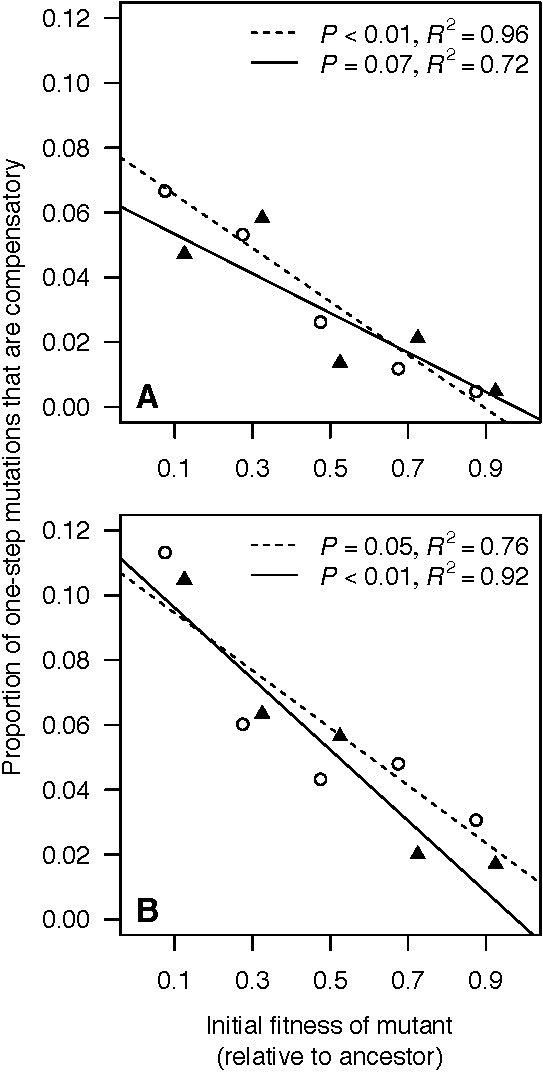
\includegraphics[width=\linewidth]{comp-avail.pdf}
\end{center}
\caption{{\bf Proportion of one-step mutations that are compensatory.}
  (A) Ancestor 1 and (B) Ancestor 2.
  %
  Open circles ($\ocircle$) and dashed lines
  represent the first mutant replicate
  while solid triangles ($\blacktriangle$) and solid lines
  represent the second mutant replicate.
  %
  Error bars are the 95\% confidence interval of the mean.}
\label{fig:comp_avail}
\end{figure}



\subsection{Effect of initial fitness of mutant}

% Perhaps have suppl. figures showing fitness increase
I evolved these 20 mutant genotypes independently
for 10,000 updates ($\sim$~850 generations)
under the same environment as the original ancestors.
%
For each genotype, the starting population
was composed of 1,000 genetically-identical individuals,
and the experimental evolution for each genotype was replicated 100 times.
%
I found that the probability of compensatory adaptation
declined with the fitness of the initial mutant
(Figures \ref{fig:W_comp}A and \ref{fig:W_comp}B).
%
In contrast, the probability of reversion
increased with the fitness of the initial mutant
(Figures \ref{fig:W_comp}C and \ref{fig:W_comp}D).
%
Note that because in some runs the fitness values decreased or did not change,
the addition of compensatory and reversion probabilities
did not always add up to 100.
%
Note also that there is a difference in the probability of compensation
for W = 0.9 between the first and second ancestor.
%
The reason for this difference appears to be that
for the first ancestor, neither compensation nor reversion
occur---the population does not change fitness.
%
This is may be due to the fact that there are few compensatory mutations
available for ancestor 1 for W = 0.9 (see Figure \ref{fig:comp_avail}).



\begin{figure}
\begin{center}
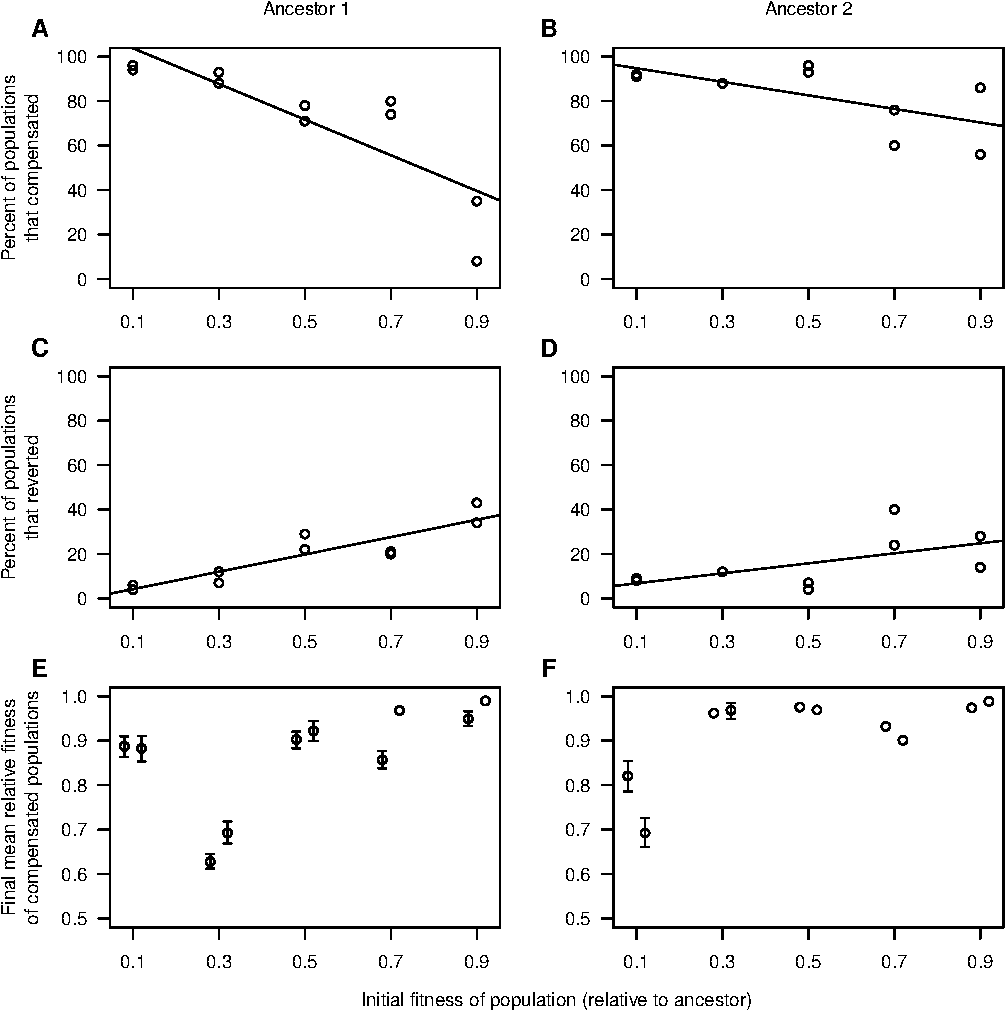
\includegraphics[width=\linewidth]{effect-W.pdf}
\end{center}
\caption{{\bf Effect of initial fitness on compensation.}
  Top figures: The proportion of runs that fully or partially compensated
  for (A) ancestor 1 (line is best fit linear model, $P =$~0.002) and
  (B) ancestor 2 ($P =$~0.043).
  Middle figures: The proportion of runs that reverted
  for (C) ancestor 1 ($P <$~0.001) and (D) ancestor 2 ($P =$~0.072).
  %Bottom figures may be irrelevant -- consider eliminating
  Bottom figures: The proportional increase in fitness for compensatory runs
  for (E) ancestor 1 and (F) ancestor 2.}
\label{fig:W_comp}
\end{figure}



There are several reasons that would explain why compensation
is higher than reversion the lower the fitness of the original mutant.
%
It is important to note that the probability
that a reversion fixes is determined by its selective advantage,
which itself depends on the fitness of the population
and on whether there is negative epistasis with current mutations.
%
The fitness of the population is initially set by the treatment
but it changes during the experiment depending on the speed of compensation.
%
The speed of compensation is directly affected by
the initial fitness of the population: the lower the initial fitness
the faster the population compensates and thus increases in fitness.
%
Negative epistasis is an intrinsic property of mutations,
but the total amount of negative epistasis is affected
by the number of mutations present when the reversion arrives.
%
This number of mutations depends on the speed of compensation
and the rate of compensatory mutations,
both of which are partly determined by the initial fitness of the population.
%
Therefore, there are both direct and indirect ways
in which the lower the initial fitness of the population
the lower the probability that a reversion fixes.



If negative epistasis was present,
the expectation is that reversion would stop being beneficial
as mutations fixed in the population.
%
The sooner reversions stopped being beneficial
the stronger that negative epistasis is with other mutations.
%
To test whether negative epistasis may have contributed in
preventing reversions from spreading in the evolving populations,
I calculated the number of generations in which a reversion
stopped being beneficial in populations that did not eventually revert.
%
First, I reverted the initial mutation to the ancestral state
for every individual in the population at each update saved
(every 100 updates or $\sim$~8.5 generations).
%
I then calculated the mean fitness of this population
relative to the mean fitness of the original population.
%
Finally, starting at the first update and continuing sequentially,
I tested whether the mean relative fitness of the reverted population
was less than 1.001; if so, reversion was no longer beneficial at this update.
%
I found that reversion stopped being beneficial sooner
at large-effect initial mutations than at small-effect initial mutations
(Figure~\ref{fig:first-update-rev-bad-W}),
indicating that negative epistasis was strongest for large-effect mutations.



\begin{figure}[b!]
\begin{center}
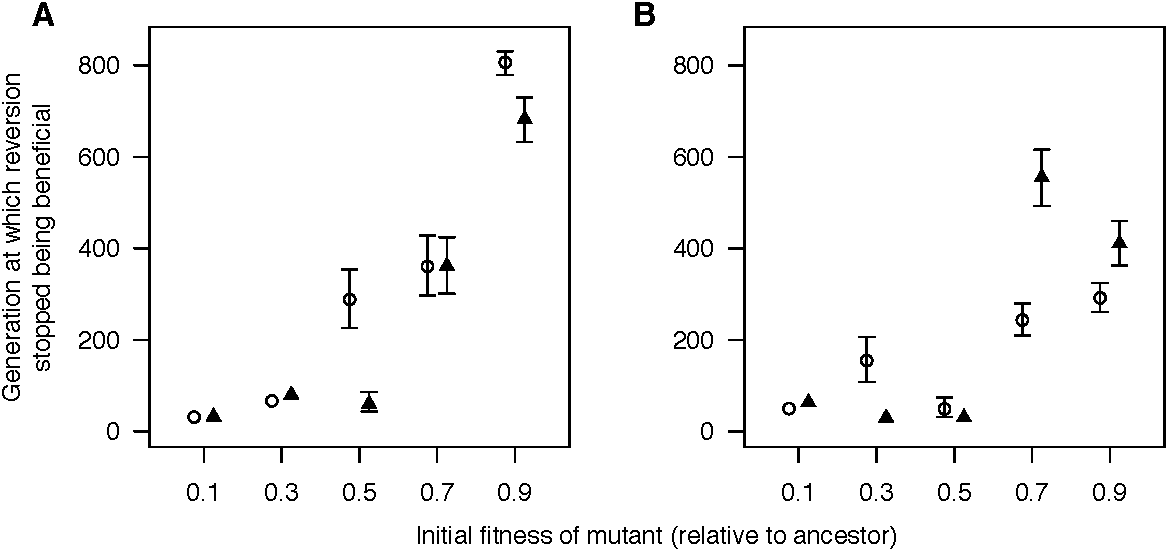
\includegraphics[width=\linewidth]{first-update-rev-bad-W.pdf}
\end{center}
\caption{{\bf Generation at which reversion stopped being beneficial
  at various initial mutant fitness effects.}
  %
  (A)~Ancestor~1 and (B)~Ancestor~2.
  %
  Open circles ($\ocircle$) and dashed lines
  represent the first mutant replicate
  while solid triangles ($\blacktriangle$) and solid lines
  represent the second mutant replicate.
  %
  Error bars are the 95\% confidence interval of the mean.}
\label{fig:first-update-rev-bad-W}
\end{figure}



As I noted before, however, the overall amount of negative epistasis
is proportional to the number of mutations accumulated.
%
Because populations that start with lower fitness adapt faster
than populations with higher fitness, they accumulate more mutations
and therefore have greater total negative epistasis.
%
In this case, negative epistasis is explained by the speed
at which compensation proceeds,
not by an intrinsic difference in negative epistasis
among treatments (i.e., initial fitness of mutant).
%
To determine whether the amount of negative epistasis
is different among treatments by accounting for the different
speeds at which compensation occurs,
I determined the number of mutations accumulated per treatment
at which reversion stopped being beneficial.
%
By examining the number of mutations accumulated
rather than the number of generations that have elapsed,
I controlled for the varying number of mutations
that accumulated through time for each treatment.
%
I still found that reversion stopped being beneficial sooner
for large-effect initial mutations than for small-effect initial mutations
(Figure~\ref{fig:first-mut-rev-bad-W}),
indicating that negative epistasis was strongest for large-effect mutations.



\begin{figure}[b!]
\begin{center}
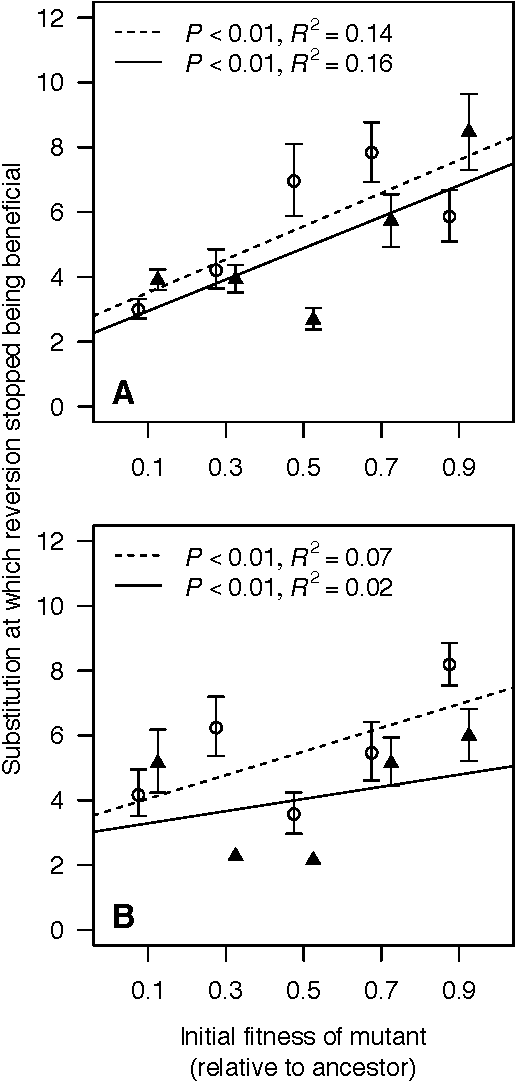
\includegraphics[width=\linewidth]{first-mut-rev-bad-W.pdf}
\end{center}
\caption{{\bf Substitution at which reversion stopped being beneficial.
  at various initial mutant fitness effects.}
  %
  (A)~Ancestor~1 and (B)~Ancestor~2.
  %
  Open circles ($\ocircle$) and dashed lines
  represent the first mutant replicate
  while solid triangles ($\blacktriangle$) and solid lines
  represent the second mutant replicate.
  %
  Lines are linear regressions for each mutant replicate.
  %
  Error bars are the 95\% confidence interval of the mean.}
\label{fig:first-mut-rev-bad-W}
\end{figure}



To further show that negative epistasis contributed
to shortening the window of opportunity for reversion,
I estimated the time at which a reversion must appear
in order to eventually reach fixation
with and without negative epistasis (see Methods).
%
These estimates were calculated using Markov chain simulations
and the known probability of reversion and selective coefficient through time.
%
I then compared these results with runs in which reversion did occur.
%
If the estimates calculated in the presence of negative epistasis
match the actual runs better than the estimates calculated without epistasis,
then I can be sure that negative epistasis
was an important contributor to slowing down the rate of reversion.
%
Indeed, I found that the actual runs matched the estimates
that were calculated in the presence of negative epistasis
(Figure~\ref{fig:expected-rev}).
%
Without negative epistasis, a reversion may appear late in evolution
and still reach fixation because its selective benefit lasts longer.
%
With epistasis, however, the window of opportunity was small,
so a reversion must appear early on if it will fix,
which was exactly what I observed in the actual runs that reverted.



\begin{figure}[th!]
\begin{center}
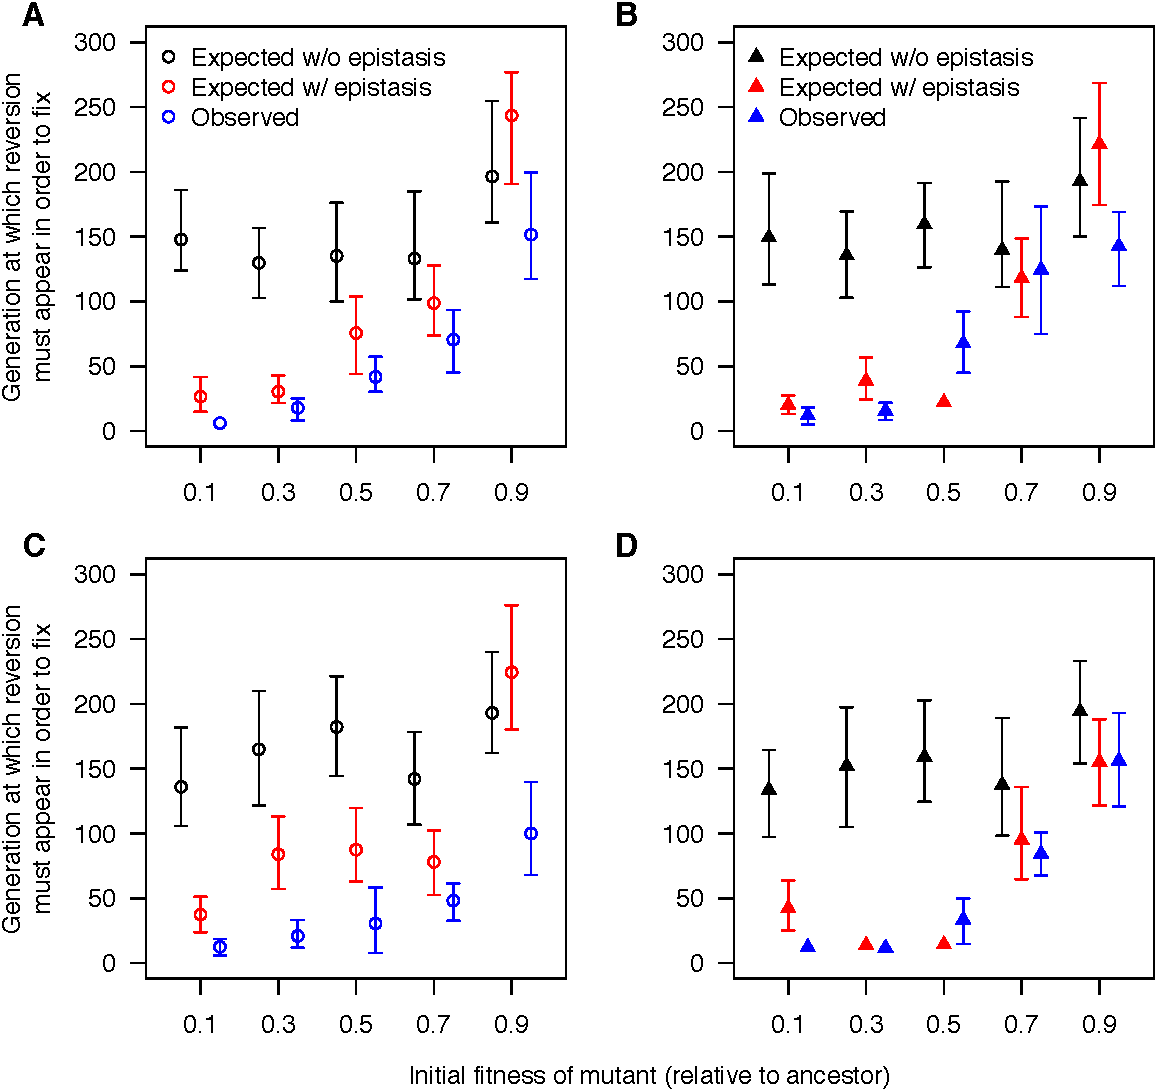
\includegraphics[width=\linewidth]{expected-rev.pdf}
\end{center}
\caption{{\bf Generation at which reversion must appear in order to fix.}
  (A)~Ancestor~1, Mutant~1, (B)~Ancestor~1, Mutant~2,
  (C)~Ancestor~2, Mutant~1, and (D)~Ancestor~2, Mutant~2.
  %
  Open circles ($\ocircle$) represent the first mutant replicate
  while solid triangles ($\blacktriangle$)
  represent the second mutant replicate.
  %
  Error bars are the 95\% confidence interval of the mean.}
\label{fig:expected-rev}
\end{figure}



I have learned that the probability of compensation and reversion
depends on the probability of finding these different kinds of mutations.
%
I should therefore expect that the population size,
which increases the total number of mutants available,
should play an important role in the probability of compensation.
%
I know that reversion is more likely to occur if it appears early
because compensatory mutations have not had an opportunity
to decrease the fitness effect of reversion
and because they have not incurred negative epistasis with reversion.
%
In large populations, the opportunity for a reversion to appear early
is higher, thus larger populations should revert more often.
%
I next examine the effect of population size on the probability
of compensation and reversion.



\subsection{Effect of population size}

I evolved the four mutants with relative fitness of 0.5
under four population sizes each: 10, 100, 1,000, and 10,000.
%
Each of these 16 experiments was replicated 100 times,
starting with a full population of genetically-identical individuals,
and evolved for 10,000 updates ($\sim$~850 generations).
%
The mutation rate was set to 0.1 mutations per generation for each experiment.
%
I found that the probability of compensatory adaptation
was highest at population sizes of 100 and 1,000
but lowest at the extremes of 10 and 10,000
(Figures \ref{fig:N_comp}A and \ref{fig:N_comp}B).
%
The probability of reversion was highest at population size of 10,000
(Figures \ref{fig:N_comp}C and \ref{fig:N_comp}D).
%
The final fitness of compensated populations
was higher the higher the population size
(Figures \ref{fig:N_comp}E and \ref{fig:N_comp}F).
%
Thus, although intermediate population sizes
had the highest probability of compensating,
they did not have the highest final fitness;
populations with size of 10,000 had the highest fitness.



\begin{figure}
\begin{center}
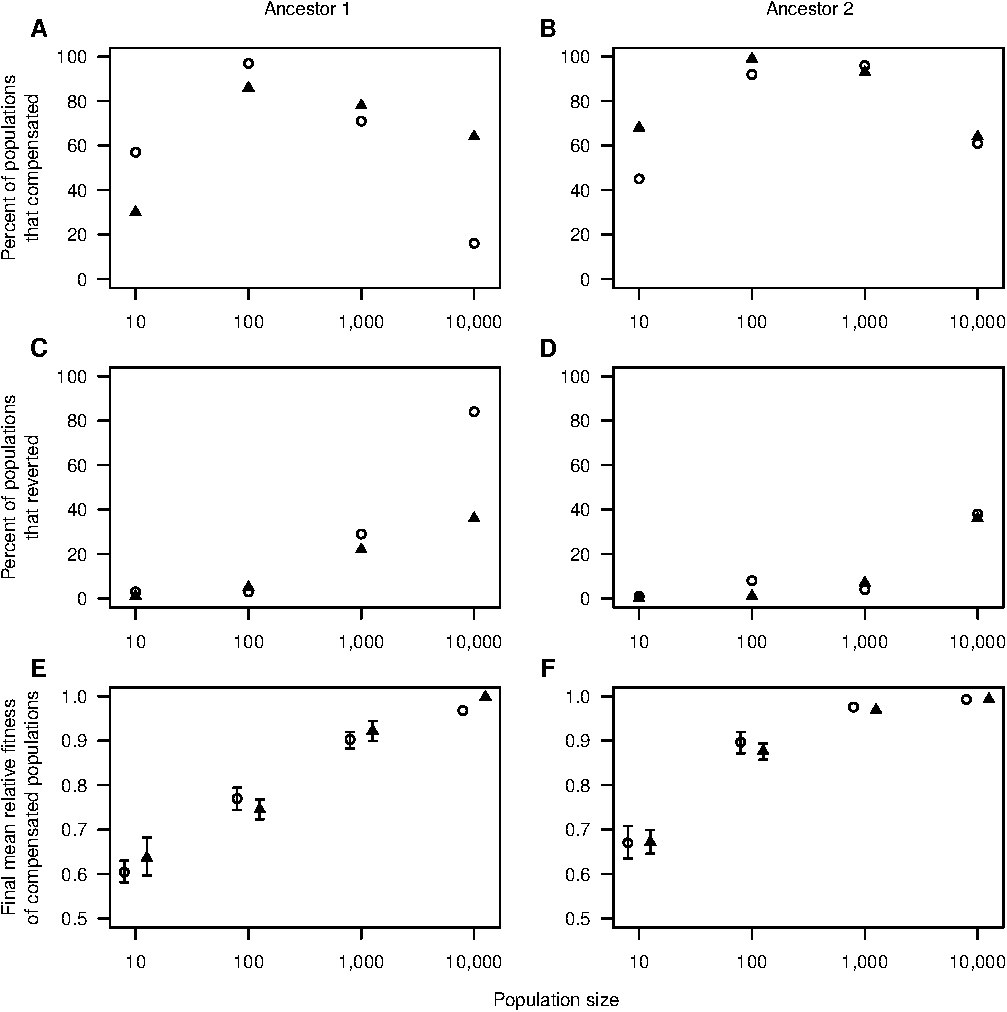
\includegraphics[width=\linewidth]{effect-N.pdf}
\end{center}
\caption{{\bf Effect of population size on compensation.}
  %
  (A) The proportion of runs that underwent compensatory evolution
  for ancestor 1 and (B) ancestor 2.
  %
  (C) The proportion of runs that reverted
  for ancestor 1 and (D) ancestor 2.
  %
  (E) The proportional increase in fitness for compensatory runs
  for ancestor 1 and (F) ancestor 2.
  %
  Open circles ($\ocircle$) represent the first mutant replicate
  while solid triangles ($\blacktriangle$)
  represent the second mutant replicate.}
\label{fig:N_comp}
\end{figure}



The reason that the probability of compensatory adaptation
at population sizes of 10,000 was lower than that at 100 or 1,000
was that the probability of reversion
at population sizes of 10,000 was higher than that at 100 or 1,000.
%
However, this did not explain the reason that the probability of compensation
at population size of 10 was lower than that at 100 or 1,000
because reversion at population size of 10 was very unlikely.
%
I observed that at population size 10
many populations decreased in fitness or did not change in fitness.
%
The number of populations that decreased in fitness
for each mutant was 27, 45, 36, and 27.
%
The number of those whose fitness stayed the same (within 1\%) was
13, 24, 19, and 9 (listed in the same order as above).
%
In contrast, for population size of 100, only 1 of them
decreased in fitness out of all 400 runs, and 8 of them stayed the same.
%
Therefore, many of the populations at size 10 that did not compensate
were accumulating deleterious mutations due to the small population size.



\subsection{Effect of mutation rate}

I evolved the four mutants with relative fitness of 0.5
under five mutation rates each: 0.0001, 0.001, 0.01, 0.1, and 1.0
(mutations per genome per generation).
%
Each of these 16 experiments was replicated 100 times,
starting with 1,000 genetically-identical individuals,
and evolved for 10,000 updates ($\sim$~850 generations).
%
The population size was kept at 1,000 throughout each experiment.
%
I found that when the mutation rate was $>$~0.0001,
the probability of compensatory adaptation
was high across the mutation rates I tested
(Figures~\ref{fig:U_comp}A and \ref{fig:U_comp}B),
except for the second mutant based on the first ancestor
(Figure~\ref{fig:U_comp}A, triangle at mutation rate 0.001),
in which 69\% of the time the population's fitness did not increase.
%
When the mutation rate was 0.0001, the probability of compensation
was low ($\sim$~20\% or less).
%
The probability of reversion increased slightly
the higher the mutation rate for the first ancestor (Figure \ref{fig:U_comp}C),
but it was generally low for the second ancestor (Figure \ref{fig:U_comp}D).
%
The final mean fitness of populations that compensated
was generally higher the higher the mutation rate,
but for the second ancestor the final fitness was lower
at a 1.0 mutation rate than that at 0.1
(Figures \ref{fig:U_comp}E and \ref{fig:U_comp}F).



\begin{figure}
\begin{center}
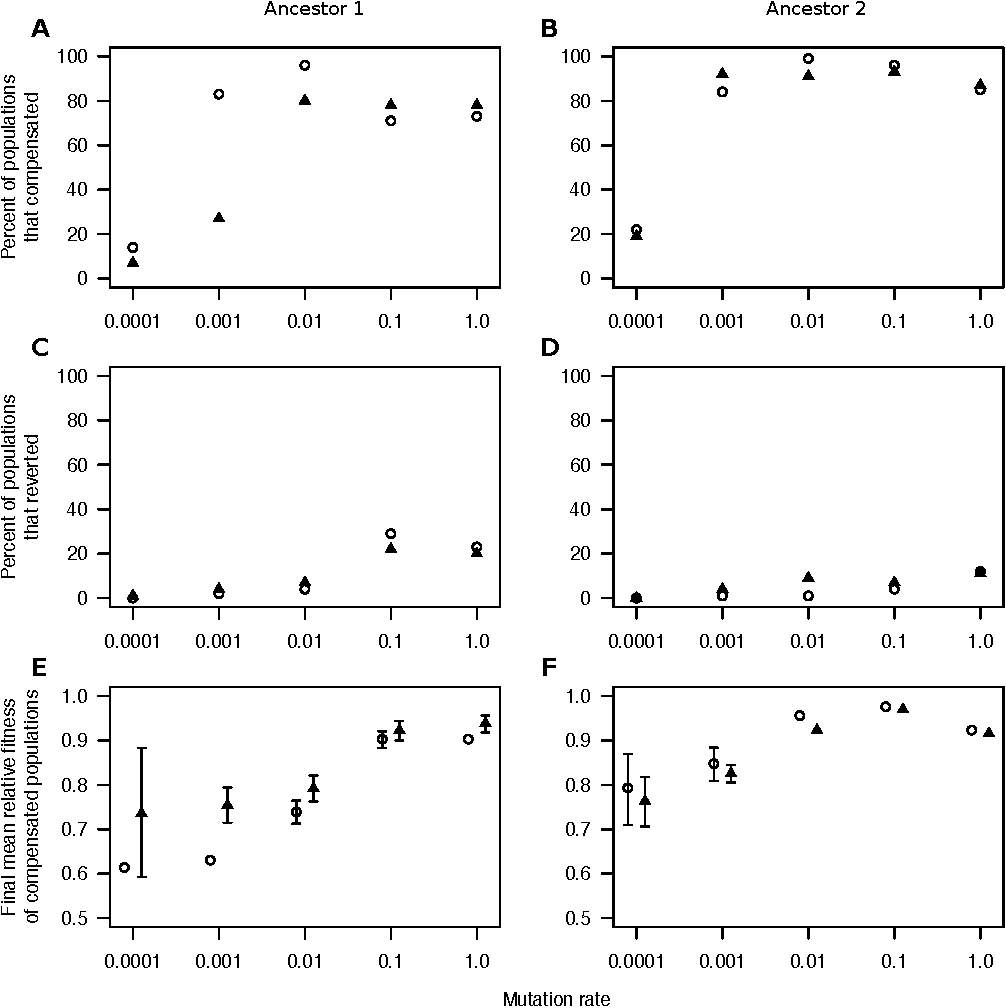
\includegraphics[width=\linewidth]{effect-U.pdf}
\end{center}
\caption{
  {\bf Effect of mutation rate on compensation, reversion,
  and final population fitness.}
  %
  Open circles ($\ocircle$) and dashed lines
  represent the first mutant replicate
  while solid triangles ($\blacktriangle$) and solid lines
  represent the second mutant replicate.
  %
  Error bars are bootstrap 95\% confidence intervals of the mean.}
\label{fig:U_comp}
\end{figure}



In our analysis of population size, reversion was highest
at the highest population size (10,000) because
the total number of mutations that arose was highest,
maximizing the likelihood that a revertant mutation appeared.
%
At the highest mutation rate (1.0),
the total number of mutations that arose was the same
as those in which the population size was 10,000
(10,000~individuals~$\times$~0.1~= 1,000~= 1,000~individuals~$\times$~1.0).
%
However, I found that reversion was less likely at a mutation rate of 1.0
(compare Figure \ref{fig:N_comp}C at population size 10,000
with Figure \ref{fig:U_comp}E at mutation rate 1.0).
%
The reason may be that at the higher mutation rate,
in which all types of mutations have a greater chance of arising,
the revertant mutation often arises on organisms with other mutations,
therefore introducing the possibility of negative epistasis.
%
To test this, I performed a similar analysis as in the initial mutation
fitness, where I calculated the number of generations in which a reversion
stopped being beneficial in populations that did not eventually revert.
%
The expectation is that the sooner reversions stop being beneficial
the stronger that negative epistasis is with other mutations.
%
I found that reversion stopped being beneficial sooner
at higher mutation rate than at lower mutation rate
(Figure~\ref{fig:first-update-rev-bad-U}),
indicating that negative epistasis was strongest at higher mutation rate.



\begin{figure}[b!]
\begin{center}
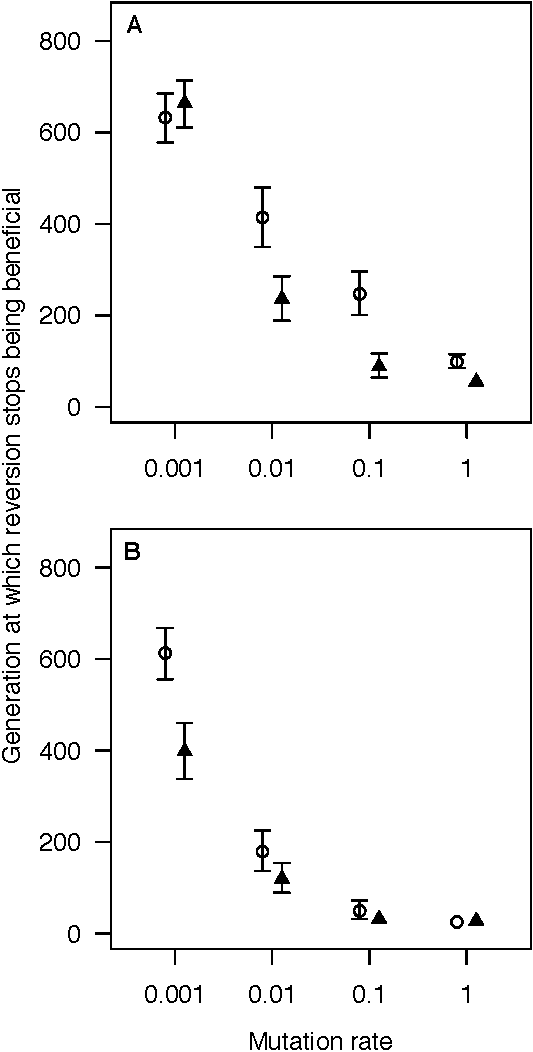
\includegraphics[width=\linewidth]{first-update-rev-bad-U.pdf}
\end{center}
\caption{
  {\bf Generation at which reversion stopped being beneficial
  at various mutation rates.}
  %
  (A)~Ancestor~1 and (B)~Ancestor~2.
  %
  Open circles ($\ocircle$) and dashed lines
  represent the first mutant replicate
  while solid triangles ($\blacktriangle$) and solid lines
  represent the second mutant replicate.
  %
  Error bars are bootstrap 95\% confidence intervals of the mean.}
\label{fig:first-update-rev-bad-U}
\end{figure}



\section{Discussion}

Our results corroborate previous findings that compensatory adaptation
is a common alternative to reversion \citep{bur99,moo00,lev00,mai02,est11}.
%
\citet{lev00} stated that ``compensatory evolution
establishes an adaptive valley that is difficult to traverse and thus return to
the ancestral genotype \ldots'' and identified two reasons for this:
(1) there are more compensatory mutations than a revertant mutation and
(2) in serial transfers, population bottlenecks hinder the spread of reversions.
%
They found in their experiments that both processes were going on: ``the rate
of compensatory mutation exceeds that of reversion by at least a factor of 10''
and 2/8 experiments reverted using a higher bottleneck but 0/12 experiments
reverted using a smaller bottleneck.
%
In our populations, there is no serial passage (like a chemostat), so I do
not have the problem of bottlenecks, although populations are limited in size.
%
Yet I see a lot of compensation, meaning that bottleneck
reason is not as important as other factors.
%
Instead, I found that negative epistasis between compensatory mutations
and a revertant (i.e., absence of the deleterious mutation)
prevented the revertant from spreading in a population.



\subsection{Availability of compensatory mutations}

\citet{moo00} and \citet{san05}
found that low-fitness mutants compensated faster than high-fitness mutants.
%
The reason was that, as \citet{moo00} explained,
a compensatory mutation in a low-fitness mutant
has a higher selective coefficient than in a high-fitness mutant
(assuming the compensatory mutation increases fitness relative to the mutant
equally for low-fitness and high-fitness mutants).
%
An alternative explanation,
which \citet{moo00} also discussed
but lacked the evidence to support it,
was that there may be more compensatory mutations available
in low-fitness mutants than in high-fitness mutants.
%
In fact, this was exactly what I found
in our digital mutants (Figure~\ref{fig:comp_avail}).
%
Our results support \citet{whi03},
who said ``when something is broken it is easier to improve than
when in is fully functional'' and \citet{poo05b},
who found a positive relationship between the negative effect
of a deleterious mutation and the probability of compensation.
%
The reason for this that \citet{poo05b} concluded was that
``deleterious mutations with large effects
on fitness may tend to affect a broader range of phenotypic components.
Severely deleterious mutations would therefore generate a larger
mutational target for compensatory interactions.''
%
This must be going on in our populations because the more severe
the deleterious mutation, the more tasks that are being knocked out.
%
I did not find, as \citet{san05} found,
that low-fitness mutants improved in fitness more than high-fit mutants
(Figures~\ref{fig:W_comp}E and \ref{fig:W_comp}F).



\subsection{Effect of initial mutant fitness}

Compensatory mutations depend upon the original deleterious mutation
they compensate, such that they may be deleterious when the deleterious mutation
is removed, such as when reversion occurs \citep{sch97,poo05,lev00}.
%
Negative epistasis between compensatory mutations and revertant mutations
prevented reversion from being beneficial earlier for low-fitness mutants
than for high-fitness mutants (Figure~\ref{fig:first-update-rev-bad-W}).
%
Reversion in low-fitness mutants may have stopped being beneficial earlier
than high-fitness mutants for two reasons.
%
The first reason may be that because in low-fitness mutants
there are many more compensatory mutations available
than in high-fitness mutants (Figure~\ref{fig:comp_avail}),
more mutations fix in low-fitness mutants \citep{moo00,san05}, so that
when a reversion appears, it does so in the genetic background
with many mutations, in which there are more chances for negative epistasis.
%
The second reason may be due to the fact that large-effect
compensatory mutations, which are more likely to fix in low-fitness mutants
cause large-effect negative epistasis.
%
I clearly see the latter reason going on: large-effect compensatory mutations
have stronger negative epistasis with the revertant mutation.
%
I cannot, however, exclude the former, and it is likely going on as well.
%
The importance of all this is that as compensatory adaptation proceeds,
it becomes increasingly harder for reversion to occur,
and populations are obligated to diverge in unique evolutionary paths
because typically there are multiple ways to compensate \citep{pau07}.
%
This decreasing probability of reversion as compensatory adaptation proceeds
has been inferred in mammalian evolution \citep{soy12}.



\subsection{Population size}

Previous studies have generally found that reversion is more common
in large populations \citep{bur99,arg07}.
%
\citet{bur99} found that in two of their large populations
(1,000 and 10,000) a single step recovered fitness substantially.
%
The single step for population 1,000 recovered fitness completely
and it may have been a revertant mutation, although this is unknown.
%
Smaller populations recovered fitness stepwise, and therefore
could not have been revertant mutations,
and their smallest populations increased in fitness very slowly.
%
Our results corroborate their findings and
those of \citet{san05} in that
the probability of reversion increased with population size
and the fitness of populations was greater the greater the population size.
%
In contrast, \citet{mai02} observed that
compensation happened more readily at greater population size
(even in the millions), and reversion was hardly observed.
%
The difference may have been due to differences in mutation rate:
viruses and our digital organisms have high mutation rates
that may have caused revertants to appear more frequently.
%
Both \citet{bur99} and \citet{mai02}
found that fitness was highest when the population size was highest,
as I did (Figures~\ref{fig:N_comp}E and \ref{fig:N_comp}F).
%
However, \citet{est03} argued that no reversion occurred in their
study at their population size of about 10,000, possibly because their mutation
rate was very low ($4.4 \times 10^{-8}$ per nucleotide per generation).



As \citet{poo00} found, compensatory mutations help ``freeze''
the mutational meltdown could have occurred in small populations.
%
But there is a limit in population size in which even compensatory adaptation
cannot save because of the overwhelming effects of drift \citep{poo05}.
%
I found that at population size of 10, many populations decreased in fitness
as they accumulated deleterious mutations.
%
Even severely deleterious populations can be compensated, and do so quickly,
but little can be done about small populations.



\subsection{Mutation rate}

\citet{mai02} found that the rate
of compensatory adaptation in \emph{Salmonella typhimurium}
was higher in a mutator strain (i.e., higher mutation rate).
%
\citet{per10} arrived at a similar result
using a mutator strain of \emph{Pseudomonas aeruginosa}.
%
Our results corroborate this trend, except at very high mutation rates,
where the probability of reversion increased and thus compensation decreased
(Figure~\ref{fig:U_comp}).
%
However, I found that the rate of reversion was not as high as expected
(based on our treatments with population size)
because the window of opportunity for reversion to be be beneficial
was very small at high mutation rates (Figure~\ref{fig:first-update-rev-bad-U}).
%
The reason was that at high mutation rates,
the revertant mutation is likely appear on a genetic background
with other mutations that could cause negative epistasis.



\subsection{Conclusions}



The fixation of compensatory mutations,
which alleviate the negative effects of fixed deleterious mutations,
is a common process in which populations recover from deleterious mutations.
%
Reversion is an alternative process,
but the competing process of compensation
dictates the window of opportunity for which reversion could happen.
%
Populations with large-effect deleterious mutations
have the most number and largest of compensatory mutations available.
%
In addition, large-effect compensatory mutations
have strong negative epistasis with the revertant mutation,
causing a smaller window of opportunity for reversion
the lower the fitness of the population.
%
Larger populations increase the probability of reversion
because there are greater chances for reversion to appear
within its widow of opportunity.
%
However, although a greater mutation rate has a similar effect,
it also shrinks reversion's window of opportunity
because other mutations are also likely to be present,
thereby causing negative epistasis.
%
Small populations and low mutation rate slow down adaptation
in general, so both compensation and reversion are less likely to occur,
but very small populations are likely to decline in fitness.



\section{Materials and Methods}



\subsection{Evolution of ancestors}

Starting with a digital organism with a genome length of 200,
I derived 20 asexual and 20 sexual ancestral populations.
%
This initial organism could reproduce but could not perform any tasks.
%
I set the grid (or `world') size to 10,000 individuals
and the point mutation rate to 0.1 per genome per generation.
%
Populations were evolved in the default nine-task environment,
re-configured to add the bonus for each task performed,
rather than multiply its power of two.
%
I allowed 20 replicate asexual populations
and 20 replicate sexual populations
to evolve for 500,000 updates ($\sim$~40,000 generations).
%
I then chose two asexual and two sexual populations
whose consensus sequence could perform all nine tasks.
%
The consensus sequences of these four populations
served as the ancestral genotypes from which mutants were derived.


\subsection{Construction and evolution of mutants}

From each ancestor, I generated every possible single mutant (5,000)
and, for the asexual ancestors, chose five pairs of mutants,
each pair with the following relative fitnesses:
0.1, 0.3, 0.5, 0.7, and 0.9 ($\pm$~0.025).
%
For the sexual ancestors, I chose two mutants
with relative fitnesses of 0.5 ($\pm$~0.025).
%
I ensured that the only allele at the mutant locus
that could fully recover fitness was the ancestral, revertant, allele.
%
If I could not find mutants with the above conditions for any ancestor,
I chose another ancestral genotype that could perform all nine tasks
and repeated the method for generating mutants.
%
In total, I obtained 24 mutants: 10 for each of the two asexual ancestors
and two for each of the sexual ancestors.


\subsection{Detection of compensatory adaptation}

To determine whether a population compensated or recovered,
I looked at the consensus sequences at the end of 10,000 updates
($\sim$~850 generations).
%
If the fitness of the consensus sequence reached 99\% of the
ancestral sequence and the allele at the mutant position
changed (to either the ancestral or to something else),
then the population was said to have reverted.
%
The reason I also considered non-ancestral alleles as reversions
is that substitutions at the mutant locus could represent
neutral alleles in the original ancestor;
this ``effective reversion'' is common in some viruses \citep{arg07}.
%
If the fitness of the consensus sequence was higher than the
mutant sequence and the allele was not the ancestral allele,
then the population was said to have compensated
(so both full and partial compensation were clumped together).
%
I included substitutions as compensations when the recovery
was partial for similar reasons as above: the mutant allele
likely has neutral mutations that are effectively equivalent.



\subsection{Estimation of the expected time for reversion}

I estimated the expected time (in updates) at which a new reversion
destined to fixation appeared.
%
To do this, I went through each update $t =$ 100, 200, \ldots, 10,000
(our data's resolution) and stopped at update $t$ with probability $p(t)$,
the probability that a new reversion appears between updates $t - 100$ and $t$
and is destined to fixation.
%
I calculated $p(t)$ as $A_{100} f(s(t))(1 - p(t - 100))$, where $A_{100}$
is the probability that a reversion appears within 100 updates,
and $f(s(t))$ is the probability that a new reversion with
selection coefficient $s(t)$ is destined to fixation (methods explained below).
%
The $1 - p(t - 100)$ is the probability that a reversion destined to fixation
did not appear in the previous update.
%
This process was repeated 100 times for each replicate run
in the treatment testing the effect of the initial fitness
(except for replicates that actually reverted because that would
interfere with calculating a reversion's selection coefficient).
%
I estimated the expected time for two different cases:
(1) the revertant's relative fitness is always 1.0 (i.e., without epistasis)
and (2) the revertant's relative fitness depends on the genetic background
on which it appears (i.e., with epistasis).



For either case, the probability $A_{100}$ that a reversion appears
within 100 updates will be the same,
but the probability of fixation $f(s(t))$ will be different because
$s(t)$ depends on whether there is epistasis.
%
To estimate $A_{100}$, I ran 100 Avida experiments where the configuration was
identical to the default experiment (except that the initial population
consisted of organisms that could not perform any tasks).
% Will readers know what the "default" experiment is?
%
During the experiments, every time a specific mutation appeared
(e.g., the position and allele of a reversion for one of our treatments),
I recorded the update at which this happened.
%
(Because the mutation rate was the same for all runs in the treatment
that tested the initial fitness, the choice of revertant to record
does not matter because the probability that any specific mutation appears
is the same for all mutations.)
%
I then binned each recorded update into bins of size 100,
counted the number in each bin, and divided that number by 100
(because there were 100 replicate runs).
%
I found that the mean of $A_{100}$ was 0.1915
with a standard deviation of 0.0443.



As mentioned before, the probability of fixation $f(s(t))$
depends on whether there is epistasis because $s(t)$ depends on this.
%
However, given a specific value of $s(t)$, call it $s$,
I can estimate its fixation probability.
%
To do this, I created every possible mutant of the first ancestor
and calculated their fitness, which gave us various values of $s$
for a revertant (calculated as $1 - w(m) / w(a)$,
where $w(m) / w(a)$ is the relative fitness of the mutant).
%
I discarded any mutants with either zero fitness
or a fitness greater than the ancestor's,
as these would result in an $s$ value less than or equal to 0
(not a beneficial reversion).
%
Then, for each unique value of $s$, I populated a new Avida world of 1,000
identical mutants and a single revertant (i.e., the ancestor).
%
(Because several different mutants sometimes had the same $s$,
I picked the first such mutant in the above configuration.)
%
I let each population run in replicates of 100 for 10,000 updates
($\sim$~850 generations) and zero mutation rate.
%
After removing one outlier, which had 1.0 fixation probability,
I fit two line segments to the data such that together they minimized
the sum of the squared residuals (the first line was anchored
at 0.001 fixation probability for $s$ of 0).
%
I found that when $s < 0.28$, $f(s) = 1.813s$
(with residual standard deviation 0.09584) and when $s \ge 0.28$,
$f(s) = 0.2414s + 0.4382$ (with residual standard deviation of 0.0643).



I estimated the revertant's selection coefficient $s(t)$
as $\overline{w}_{R}(t) - \overline{w}(t)$,
where $\overline{w}_{R}(t)$ is the revertant's mean relative fitness
and $\overline{w}(t)$ is the population's mean relative fitness
between updates $t$ and $t - 100$.
%
Because I recorded data at updates 0, 100, 200, \ldots, 10,000,
I estimated $\overline{w}_{R}(t)$ and $\overline{w}(t)$
as the mean value between those at $t$ and $t - 100$.
%
In the case where there is no epistasis, $\overline{w}_{R}(t)$ was always 1.0.
%
In the case where there is epistasis,
$\overline{w}_{R}(t)$ was the mean relative fitness of the population
where each individual in the population was given the revertant mutation.
%
These analyses were conducted for each replicate run
in which reversion did not happen (total of 1,643 runs).



\section{Acknowledgments}

This material is based in part upon work supported by
the National Science Foundation under Cooperative Agreement No. DBI-0939454.
%
Any opinions, findings, and conclusions or recommendations
expressed in this material are those of the author(s)
and do not necessarily reflect the views of the National Science Foundation.



\end{doublespace}

\bibliographystyle{apalike}
\bibliography{comp_rate}

